\section{Algorithm}
\label{sec:alg}

\begin{figure*}[t!]
\centering
  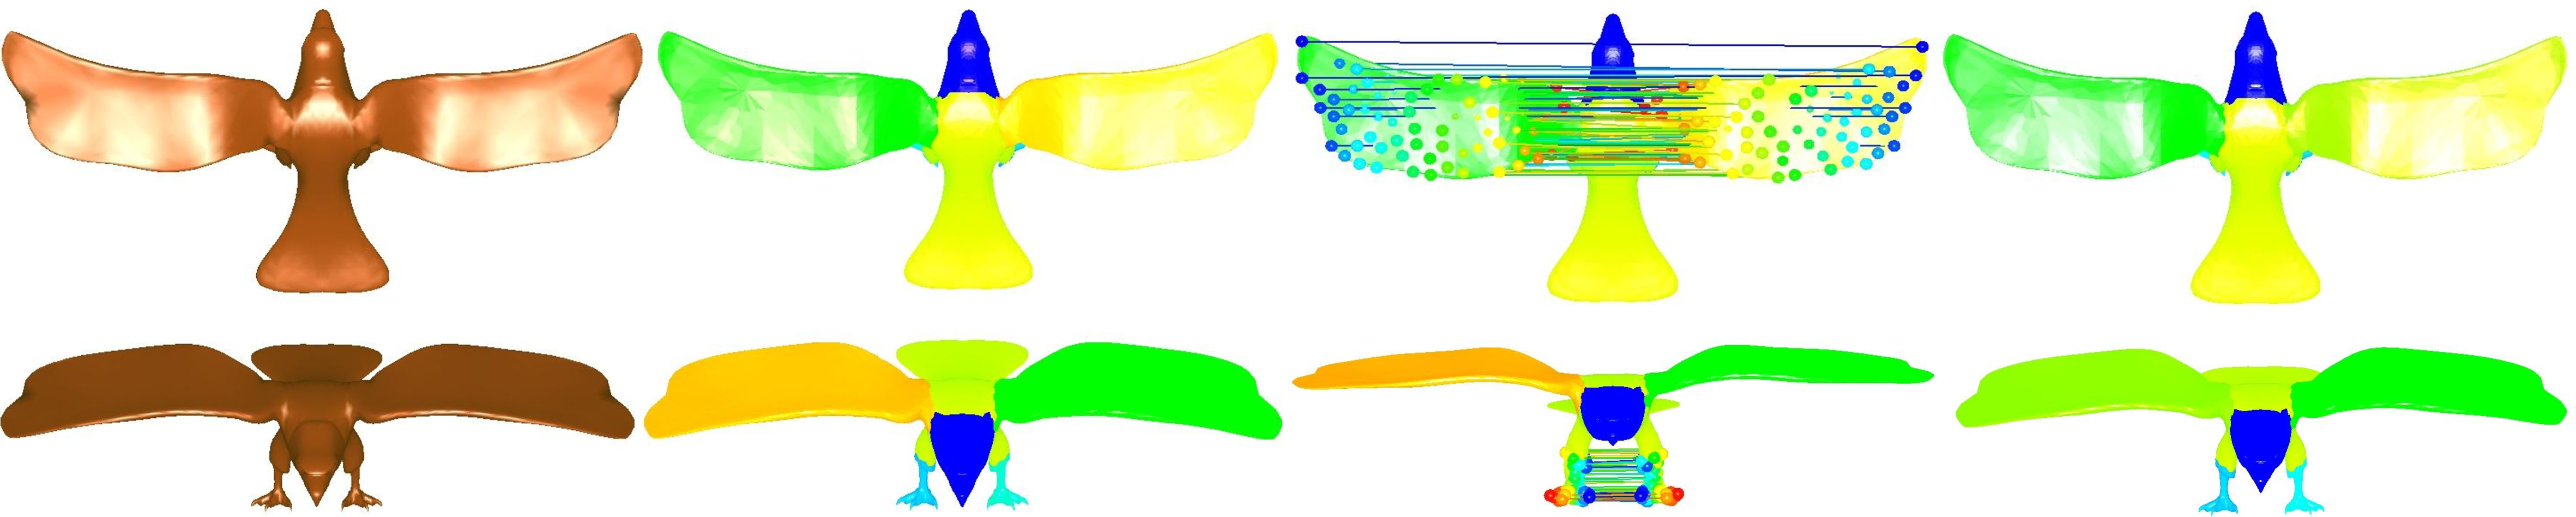
\includegraphics[width=0.99\linewidth]{figures/pipe.pdf}
  \caption{Algorithm pipeline (using an Eagle example from two viewpoints).
  Left to right: the given shape, is decomposed into several parts, each part is matched to the remaining shape, 
  and symmetry is detected by clustering the correspondences based on similarity of matching transform. }
\label{fig:Eager}
\end{figure*}


Given a shape $\mathbb{S}$, our algorithm  performs the following three steps (as illustrated in Figure~\ref{fig:Eager})
\begin{enumerate}
\item Automatically decompose the shape into parts. Implied by the existing symmetry detection algorithms~\cite{xu2009,berner2011},
      symmetric parts are always meaningful.
      This is the foundation of our algorithm and could explain why the meaningful segmentation is first performed to provide the parts for symmetry detection,
      although the other surface-based~\cite{shamir2006} segmentation algorithm could also provide the initial segmentation.
%%%RRM How do we know the segmentation boundaries will agree with the part boundaries? What happens if they
%%%RRM do not? You need to discuss this in a high level way before going into detailed subsections
%%%ZQC We would add one application on the bad segmentation, demonstrate that the effectness of segmentation.
\item For each part $\mathbb{S}_i$, match the remaining shape $\mathbb{S}-\mathbb{S}_i$ to $\mathbb{S}_i$ such that for any node in $\mathbb{S}-\mathbb{S}_i$,
      a partial match from $\mathbb{S}_i$ is performed.
%%%RRM Partial in what way? part of Si matches the rest? If so, how does Si help
\item Put together all the correspondences to form a many-to-many correspondence in $\mathbb{S}$, and cluster nodes in $\mathbb{S}$ based on similarity of local matching transformation.
\end{enumerate}
%%%RRM You need much more discussion here to
%%%RRM - justify the approach (why does segmentation help)?
%%%RRM - say what form the output takes
%%%RRM - discuss other issues above


\subsection{Automatic part-type segmentation}
\label{subsec:segmentation}
%%%RRM Why do you say meaningful? In what sense meaningful?
%%%RRM I dont see any reason to call it meaningful.

We start by decomposing the input shape $\mathbb{S}$ into $n$ parts: $\mathbb{S}_1$, $\mathbb{S}_2$, $\dots$, $\mathbb{S}_n$.
%%%RRM How and why is n chosen?
The segmentation should ideally lead to each region representing a meaningful part of the object. We use a random-walk-based part-type segmentation approach~\cite{lai2009} which starts by distributing $n$ seeds as widely as possible over the surface.
%%%RRM meaningful segmentation would put seeds in carefully chosen places, not random ones.
Each face of the  shape is assigned the label belonging to the seed which has the maximum probability of being reached by a random walk starting from the face. The probability of stepping across face edges is derived from the local geometry such that it is more difficult to move across sharp edges.
%%%RRM The rest of this paragraph does not make sense.
%%%RRM I agree that symmetric parts are meaningful.
%%%RRM However, there is nothing special about our segmentation
%%%RRM that makes it "meaningful" or specially suited to symmetry detection.
%%%RRM There is nothing in this section saying WHY you do segmentation, and how you are going to USE
%%%RRM the segmentation results.

\subsection{Region matching}
\label{subsec:matching}

%%%RRM There is nothing in this section to relate the regions to the segmentation.
%%%RRM You also need to explain how this fits into the overall problem:
%%%RRM how does region matching help to find symmetries?

In order to find the symmetries, we uniformly sample the shape $\mathbb{S}$ with $m$ sample regions,
%%%RRM what is a sample region? Do these cover the shape?
%%%RRM How big are the sample regions? How is sampling related to the segmentation?
and then build the partial matching between every pair of regions $\mathbb{S}_i$ and $\mathbb{S}_j$, $i \neq j$. Typically we set $m=100 n$.
%%%RRM Why?
%%%RRM Explain what you mean by a partial matching. What is the partial matching looking for, what
%%%RRM form does the output take?

Partial matching is performed using a third-order tensor matching algorithm [reference omitted for review].
Our algorithm formulates the matching using a supersymmetric tensor representing an affinity metric,
which takes into account feature similarity and geometric constraints between features.
Matching is performed by an efficient higher-order power iteration approach which takes advantage of the compact representation of the supersymmetric affinity tensor; an efficient sampling strategy is used to compactly estimate the affinity tensor.
%%%RRM Too much about previous work. Omitted.

The algorithm matches point triples from each shape, taking into account geodesic distances between points.
%%%RRM What feature vector is used at each point?
To compute geodesic distances, the approximate Dijkstra algorithm~\cite{Dijkstra1959} is used.
Suppose the number of matches between regions $\mathbb{S}_i$ and $\mathbb{S}_j$ is $M_{i,j}$.
These regions are recognized as a candidate symmetry if $M_{i,j} > c m$, where $c$ is a constant and set to $0.2/n$
for all examples in the paper.


\subsection{Correspondence clustering}

%%%RRM Now say WNY clustering is used (presumably to put together the region matches into bigger
%%%RRM consistent matches representing symmetries).

Next, we gather together all correspondences for each part $\mathbb{S}_i$, found by the partial matching, giving many-to-many correspondences for the whole of $\mathbb{S}$.
Then, we cluster correspondences based on local transformation consistency of the matching.

For each partial matching output a rigid transform can be computed from each triple of compatible matching points, following~\cite{Huttenlocher1990}.
As shown by ~\cite{Huttenlocher1990}, this transformation always exists for three non-collinear points, and is unique up to a reflective ambiguity.
The solution is in closed-form and only involves second-order equations, so it is run in the fast speed.

For all sampled points, our clustering method is performed similar to the one used in~\cite{mitra2006}, which determines transformations that map local surface patches onto each other.
Each matching pair provides evidence for a symmetry relation at the level of the local sample spacing.
From these, we extract meaningful symmetries at larger scales by finding groups of pairs with a similar transformation that correspond to symmetric subsets of the shape.
We use mean shift clustering~\cite{Comaniciu2002} for this purpose, a non-parametric method based on gradient ascent on a density function.
The corresponding symmetry transformation is then defined by the cluster��s maximum. 
Please note that, as observed by Mitra et al.~\cite{mitra2006}, the significant modes detected by the mean-shift clustering algorithm do not necessarily correspond to a meaningful symmetry.
So, we also make use of the similar verification step~\cite{mitra2006} to compute the accurate symmetry regions.
But our spatial consistency is also constrained by the former segmentation results. 
For more details on mean-shift clustering and verification we refer to~\cite{mitra2006}.  

\subsection{Segmentation-and-symmetry iteration}
\label{subsec:iteration}

Until now, one complete segmentation-based symmetry detection processing has been presented. 
As the initial segmentation does not often produce accurate meaningful part, the symmetry detection also is also not so perfect.
So, the further refinement should be performed both on the segmentation and symmetry.
Fortunately, as shown in Figure~\ref{fig:Gargoyl} top, the initial symmetry detection could detect accurate mirroring symmetry.
The useful symmetry result could be further used to refine the segmentation, then improve the symmetry as a result.
The symmetry information is used as the guide to place the seed points in the random-walk-based segmentation algorithm~\cite{lai2009}.
For the seeds at the Garoyl statues, two are placed at the symmetric left and right wings, same as those at the left and right bodies.
Besides, one is placed at the head, and the last is place at status base.
Beyond the seeds placement, the better segmentation could be produced as the center-left as~\ref{fig:Gargoyl}.
Consequently, based on the better segmentation, the better symmetry is further detected as the center-right.






